% EE2000 Preliminary Report -- revised version
% Template: IEEE/CVF (cvpr.sty). Keep your course-provided cvpr.sty and
% ieeenat_fullname.bst next to this file.
%
% Search for "TODO" and for square-bracketed text ([...]) before
% submitting: those are items only you can fill in or confirm.

\documentclass[10pt,twocolumn,letterpaper]{article}

% Non-review mode so that the team is identifiable. If your cvpr.sty does
% not accept the pagenumbers option, use \usepackage{cvpr} instead.
% \usepackage[pagenumbers]{cvpr}
\usepackage[review]{cvpr} 


\usepackage{graphicx}
\usepackage{amsmath}
\usepackage{amssymb}
\usepackage{booktabs}
\usepackage{tabularx}
\usepackage{tikz}
\usetikzlibrary{arrows.meta,positioning,fit,backgrounds}

\usepackage[pagebackref,breaklinks,colorlinks,allcolors=cvprblue]{hyperref}
\def\paperID{15}
\def\confName{EE2000}
\def\confYear{2026}

\title{Real-Time EEG Seizure Detection Using Discrete Wavelet Transform\\
and Support Vector Machine on FPGA}

% TODO: fill in the four team members (names and roll numbers) and team ID.
\author{[Member A, roll no.] \quad [Member B, roll no.]\\[2pt]
[Member C, roll no.] \quad [Member D, roll no.]\\
Team [ID], EE2000 Signal Processing, IIT Hyderabad}
\definecolor{cvprblue}{rgb}{0.21,0.49,0.74}
\usepackage[pagebackref,breaklinks,colorlinks,allcolors=cvprblue]{hyperref}
\begin{document}
\maketitle

%---------------------------------------------------------------------
\begin{abstract}
Automatic detection of epileptic seizures from scalp
electroencephalography (EEG) is a nonstationary, heavily class-imbalanced
signal-processing problem in which detection sensitivity, false alarms,
and latency must be balanced together. This report proposes an
FPGA-based, streaming seizure-detection pipeline for the Boolean Board
(Xilinx Spartan-7) that band-limits an EEG stream, applies a
Daubechies-4 discrete wavelet transform (DWT), accumulates wavelet-domain
features over sliding windows, and classifies each window with a linear
support vector machine (SVM), followed by temporal post-processing that
requires consecutive positive windows before raising an alarm. The
primary dataset under consideration is the CHB-MIT Scalp EEG Database
from PhysioNet. This is a preliminary report: it states the problem,
reviews related work (software and hardware seizure detectors, including
FPGA and ASIC implementations), explains why published results obtained
under different evaluation protocols cannot be compared directly, and
sets out a staged plan. No experimental or hardware results are reported
here; the design parameters (channel count, window length, DWT level,
feature set, word length, evaluation protocol) are working baselines to
be finalized after dataset analysis and software baselining.

\medskip
\noindent\textbf{Keywords:} EEG, seizure detection, epilepsy, discrete
wavelet transform (DWT), support vector machine (SVM), FPGA, real-time
signal processing, class imbalance, medical device.
\end{abstract}

%---------------------------------------------------------------------
\section{Introduction}
\label{sec:intro}

Scalp EEG records the summed electrical activity of large neuronal
populations as microvolt-level voltage differences between electrodes.
Seizure activity typically appears as rhythmic, multi-component activity
whose spectral content, spatial distribution, and time course differ
between patients and even between seizures of the same patient
\cite{shoeb2010icml}. Detecting seizure onset automatically is therefore
a signal-processing problem before it is a clinical one: a detector must
separate seizure activity from normal background rhythms, sleep
spindles, and artifacts, using short segments of a noisy, multi-channel,
nonstationary signal.

Four properties make the problem difficult. First, EEG is nonstationary:
its statistics change within and between the seizure and non-seizure
states, and a single seizure can evolve in amplitude and frequency over
a few seconds \cite{shoeb2010icml}. Second, the signal is noisy and
contaminated by non-cerebral artifacts. Third, seizure-related events
are transient, so a detector must react to short-lived patterns. Fourth,
there is strong inter-patient variability: EEG that indicates a seizure
in one patient can resemble a benign pattern in another
\cite{shoeb2010icml}. These properties motivate time--frequency analysis
rather than a single global spectrum.

The discrete wavelet transform (DWT) is a natural candidate. It
decomposes a signal with a multiresolution filter bank, giving
coarse-to-fine sub-bands with time localisation \cite{mallat1989theory}.
The Daubechies family of compactly supported orthonormal wavelets
\cite{daubechies1988orthonormal} appears widely in the EEG literature,
including the db4 wavelet \cite{shen2022dwt,subasi2007eeg}. % TODO: confirm Subasi's wavelet choice
Statistics of the wavelet coefficients (for example, energy per
sub-band) can then be passed to a classifier such as a support vector
machine (SVM) \cite{cortes1995support}.

\paragraph{Why implement this on an FPGA?} An FPGA is not required for
EEG at 256\,Hz: as Sec.~\ref{sec:fpga} shows, the arithmetic load is
tiny and a conventional microcontroller would also suffice. The
motivation is primarily engineering. The pipeline is a regular,
multiply--accumulate-dominated streaming design, so the FPGA serves as a
testbed for quantization and resource profiling, deterministic latency,
and bit-exact verification against a software model.
Sec.~\ref{sec:fpga} discusses these advantages and limitations.

\paragraph{Target platform.} The Boolean Board is an educational board
built around a Xilinx Spartan-7 XC7S50 FPGA; according to the
manufacturer's reference manual the device provides 120 DSP blocks and
337\,KB of block RAM, and the board offers a USB UART, 16 LEDs, and an
eight-digit seven-segment display \cite{realdigital2024boolean}. These
resources are sufficient in principle for a dataset-playback
demonstration with visual alarm output. Whether the full pipeline fits,
and at what clock rate, is an open question that this project will
measure.

\paragraph{Contribution and scope.} This project is best described as an
engineering-oriented replication and integration effort. FPGA and ASIC
seizure detectors already exist (Sec.~\ref{sec:hw}); we do not claim
algorithmic novelty. The intended value lies in a reproducible,
streaming FPGA implementation of a literature-grounded DWT +
linear-SVM pipeline, validated against a Python reference model,
evaluated on an established benchmark, and demonstrated on the Boolean
Board with dataset playback. The demonstration is not a medically
validated device and makes no clinical claim.

\subsection{Problem statement}
\label{sec:problem}

The project aims to design, implement, and evaluate a real-time
FPGA-based EEG seizure-detection pipeline. Formally, for a datapath word
length $B$ and classifier and pipeline parameters $\theta$, we frame this
as a hardware-constrained optimization problem:
\begin{equation}
\begin{aligned}
\max_{\theta,B}\;& \mathrm{Sens}(\theta,B)\\
\text{s.t.}\;& \mathrm{FA/h}(\theta,B)\le\epsilon,\quad L(\theta,B)\le\tau,\\
& N_{\mathrm{DSP}}(B)\le 120,\quad M_{\mathrm{BRAM}}(B)\le M_{\max},
\end{aligned}
\label{eq:problem}
\end{equation}
where $\mathrm{Sens}$ is event sensitivity, $\mathrm{FA/h}$ is the
false-alarm rate, $L$ is mean detection latency, and $N_{\mathrm{DSP}}$
and $M_{\mathrm{BRAM}}$ are the DSP and block-RAM usage against the
limits of the Spartan-7 XC7S50. Eq.~\eqref{eq:problem} is a framing, not
a problem we solve jointly: the SVM weights are trained offline by
regularized hinge-loss minimization, while $B$ and the post-processing
parameter $k$ are swept, and $N_{\mathrm{DSP}}$ and $M_{\mathrm{BRAM}}$
also depend on channel count and scheduling. The targets $\epsilon$ and
$\tau$ will be fixed after software baselining; for reference,
\cite{shoeb2010icml} reports about two false detections per 24\,h
($\approx0.08$/h) and a median delay of 3\,s under its own protocol.
Performance will be evaluated under an explicitly stated protocol
(Sec.~\ref{sec:protocol}).

%---------------------------------------------------------------------
\section{Dataset Under Consideration}
\label{sec:dataset}

The primary dataset under consideration is the CHB-MIT Scalp EEG
Database, hosted by PhysioNet \cite{guttag2010chbmit,goldberger2000physionet}
and introduced with the work of Shoeb and colleagues
\cite{shoeb2009thesis,shoeb2010icml}. The following facts are taken from
the official PhysioNet description \cite{guttag2010chbmit}.
% TODO: confirm these counts against the PhysioNet page, RECORDS and
% SUBJECT-INFO (198 seizures vs 182 in the original 23 cases suggests
% different subsets of the collection).
\begin{itemize}
  \item The database contains EEG from pediatric subjects with
    intractable seizures, recorded at Children's Hospital Boston.
    Recordings are grouped into 23 cases from 22 subjects; case chb21
    was obtained 1.5 years after chb01 from the same female subject.
  \item All signals were sampled at 256 samples/s with 16-bit
    resolution, using the international 10--20 electrode system.
  \item The collection lists 664 \texttt{.edf} files, of which 129
    contain one or more seizures. In all, the records include 198
    seizures (182 in the original 23 cases); seizure onset and end are
    annotated.
  \item Files usually hold one hour of signal, though some cases use
    two- or four-hour files. There are occasional gaps between
    consecutive files, usually 10\,s or less.
  \item The total uncompressed size is 42.6\,GB.
\end{itemize}

Channel layout is not uniform. Most files contain 23 EEG signals, but 24
or 26 in a few cases; up to five ``dummy'' signals (named ``-'') are
interspersed among the EEG signals; and some records include non-EEG
signals, such as an ECG channel in the last 36 files of case chb04 and a
vagal-nerve-stimulus channel in the last 18 files of chb09
\cite{guttag2010chbmit}. The montage for each recording is documented in
the per-case summary files. Consequently, the recordings must not be
assumed to share a common montage. Choosing a channel subset that is
present and consistently named across the recordings actually used---or
a per-patient selection---is an early and consequential decision. It
sets the feature-vector dimension, the classifier size, and, on the
FPGA, how many channels the datapath must serve. This decision is
deferred to the dataset-inspection stage (Sec.~\ref{sec:next}).

\paragraph{Caution on quoted figures.} Published papers describe this
dataset in slightly different ways (for example in the number of
subjects or hours used), because each study selects its own subset.
Where we cite results we therefore state the subset or protocol the
authors used, and we take dataset statistics only from the official
documentation above.

%---------------------------------------------------------------------
\section{Literature Review}
\label{sec:lit}

This section is organised from general to specific: software detectors,
wavelet methods, features, classifiers, and finally hardware
implementations. Published results are attributed to their sources and
are not our results.

\subsection{Conventional and machine-learning seizure detection}

Shoeb and Guttag \cite{shoeb2010icml} frame seizure-onset detection as a
binary classification problem on short EEG epochs, and their work
accompanies the CHB-MIT database. They slide a 2\,s window over the
signal, pass each channel through a filter bank spanning 0.5--25\,Hz, and
measure the energy in each passband. Energies from 18 channels are
concatenated into a spatial--spectral vector (with 8 filters, 144
elements), and vectors from three consecutive windows are stacked to
capture temporal evolution. An SVM with an RBF (non-linear) kernel
performs classification. Trained on two or more seizures per patient and
tested on 916 hours of continuous EEG from 24 patients (23 pediatric
plus one adult patient), the authors report detection of 96\% of 173
test seizures, a median detection delay of 3\,s, and a median
false-detection rate of two per 24 hours; the mean latency was 4.6\,s.
Two details matter for our purposes. The evaluation is patient-specific
and uses leave-one-record-out cross-validation, and the authors
explicitly caution that leaving out short epochs instead of whole
records gives misleadingly good results, because neighbouring epochs are
strongly correlated. They also compare against a patient non-specific
commercial detector, which they report detected 61\% of seizures with 33
false detections per 24 hours on the same data. Because that detector
differs in algorithm as well as in patient-specificity, the gap should
not be attributed to patient-specificity alone.

The earlier patient-specific work of Shoeb et al. \cite{shoeb2004patient}
is cited by PhysioNet as related prior work.

\subsection{Wavelet-based seizure detection}

Wavelets suit EEG because the signal is nonstationary and seizure
activity is transient. The DWT computes a pyramidal decomposition using
conjugate mirror filters (often loosely called quadrature-mirror
filters) \cite{mallat1989theory}: at each level a low-pass filter
produces an approximation and a high-pass filter produces detail
coefficients, each decimated by two. For an input $x[n]$ with low-pass
filter $h[\cdot]$ and high-pass filter $g[\cdot]$,
\begin{align}
a_{j+1}[k] &= \sum_n h[n-2k]\,a_j[n], \\
d_{j+1}[k] &= \sum_n g[n-2k]\,a_j[n],
\end{align}
with $a_0[n]=x[n]$. The Daubechies family provides compactly supported
orthonormal wavelets with a chosen number of vanishing moments
\cite{daubechies1988orthonormal}; db4 has an eight-tap filter pair. Its
compact support keeps the hardware filters short.

Sub-bands are only approximate frequency partitions. For a sampling rate
$f_s$, the detail sub-band at level $j$ nominally covers
$[f_s/2^{j+1},\,f_s/2^{j}]$ and the final approximation covers
$[0,\,f_s/2^{J+1}]$ for $J$ levels, but the filters have transition
bands and overlap, so the partition is not a sharp division. At
$f_s=256$\,Hz a 5-level decomposition nominally gives detail bands near
64--128, 32--64, 16--32, 8--16 and 4--8\,Hz and an approximation near
0--4\,Hz. These ranges resemble but do not coincide with the clinical
delta/theta/alpha/beta bands, so we treat the sub-bands as data-driven
features rather than as exact physiological rhythms. If the signal is
band-limited to about 25\,Hz, the two finest detail bands carry little
seizure-relevant energy and may be dropped from the feature vector.

In the literature, wavelet features are used widely. Subasi
\cite{subasi2007eeg} studies DWT-derived statistics for EEG
classification on a different dataset from CHB-MIT; we cite it only as an
example of wavelet features for EEG.
% TODO: check which wavelet Subasi found best before making any db4 claim.
Shen et al. \cite{shen2022dwt} use DWT with eight eigenvalue (feature)
algorithms on two public datasets, a short-term dataset from the
University of Bonn and CHB-MIT. Per the publisher abstract, an SVM is
used for a three-class task (healthy, seizure-free, seizure-active) on
the Bonn data, whereas the real-time onset detection on CHB-MIT uses a
RUSBoosted tree ensemble. The authors report 96.38\% accuracy, 96.15\%
sensitivity and a 3.24\% false-positive rate on CHB-MIT. Their
highlights mention DB4 and DB16 wavelets; from the accessible text, the
CHB-MIT experiment uses DB16 with 7 features. Because the full text was
not accessible to us, details such as channels, window length and
train/test split are marked ``Not verified'' in Table~\ref{tab:lit}.

\subsection{Feature extraction and statistical descriptors}
\label{sec:features}

Hardware detectors favor features that are inexpensive to compute in
streaming form, relying on multiply--accumulate (MAC) or add--accumulate
operations and avoiding square roots, divisions and logarithms. For a
sub-band $b$ with $N_b$ coefficients $c_i$ in the current window
($N_b = T f_s/2^{j}$ for a window of $T$ seconds at detail level $j$),
we consider two primary features, the sub-band energy and the
line-length:
\begin{align}
  E_b &= \frac{1}{N_b}\sum_{i=1}^{N_b} c_i^{2}, \label{eq:energy}\\
  \mathrm{LL}_b &= \frac{1}{N_b-1}\sum_{i=2}^{N_b} \left| c_i - c_{i-1} \right|. \label{eq:ll}
\end{align}
Sub-band energy is widely used for EEG seizure detection, including in
the original CHB-MIT detector \cite{shoeb2010icml}, and several of the
reviewed designs use wavelet-domain features (Table~\ref{tab:lit}).
Line-length was proposed as an efficient seizure-onset feature in
\cite{esteller2001}; we include it because it responds to both amplitude
and frequency changes while needing only a subtraction, an absolute
value and an accumulator.

The variance
\begin{equation}
  \sigma_b^{2} = E_b - \mu_b^{2}, \qquad
  \mu_b = \frac{1}{N_b}\sum_{i=1}^{N_b} c_i,
\end{equation}
is a candidate only. For detail sub-bands the mean $\mu_b$ is
approximately zero, so $\sigma_b^{2}\approx E_b$ and the two features
are nearly redundant; we therefore omit the variance (and the standard
deviation, which additionally needs a square root) unless the software
baseline shows a benefit.

\paragraph{Hardware cost.} Both features reduce to a single accumulator
per sub-band. The normalizations $1/N_b$ and $1/(N_b-1)$ are constants
per sub-band, so they can be absorbed into the SVM weights offline (or,
when $N_b$ is a power of two, implemented as a shift). For $B$-bit
wavelet coefficients, the energy accumulator must hold
$2B+\lceil\log_2 N_b\rceil$ bits, since squaring doubles the word length
before the sum adds $\log_2 N_b$ bits of growth. The line-length
accumulator needs only $B+1+\lceil\log_2 N_b\rceil$ bits. Truncating the
products before accumulation trades accumulator width against error, and
will be part of the word-length study (Sec.~\ref{sec:arch}). The feature
vector has dimension $D = C\, n_b\, n_f$ for $C$ channels, $n_b$
sub-bands and $n_f$ features per sub-band, which sets the size of the
linear SVM.

\paragraph{Feature scaling.} Raw sub-band energies are heavy-tailed and
can span several orders of magnitude. Per-patient linear standardization
(subtracting a mean and dividing by a standard deviation, both computed
offline) can be folded into $\mathbf{w}$ and $b$ of the SVM at no
hardware cost. A logarithmic transform cannot be folded in, and is not a
plain MAC operation; it could be approximated in hardware with a
leading-zero counter and a small lookup table. Whether a log transform
improves classification enough to justify this cost will be decided in
the software baselining phase.

\subsection{Machine-learning classifiers and why a linear SVM}

The SVM \cite{cortes1995support} constructs a maximum-margin decision
surface. For a feature vector $\mathbf{x}\in\mathbb{R}^{D}$, a linear SVM
decides by
\begin{equation}
  \hat{y}=\operatorname{sign}\!\left(\mathbf{w}^{\top}\mathbf{x}+b\right),
\end{equation}
where $\mathbf{w}$ and $b$ are learned offline. Inference is one dot
product, a bias addition, and a sign test: $D$ multiply--accumulates
with fixed cost, constant latency, and no data-dependent branching. That
makes it attractive for FPGA deployment, since the weights can be stored
in block RAM as fixed-point words and the computation can be pipelined
or time-multiplexed.

There is a trade-off. Non-linear (e.g., RBF) SVMs can model curved
decision boundaries: the original CHB-MIT detector uses an RBF kernel
\cite{shoeb2010icml}, and hardware designs such as Feng et al.
\cite{feng2018vlsi} implement non-linear SVMs with a Gaussian kernel.
But the cost of evaluating a kernel SVM grows with the number of support
vectors, which is data-dependent. Small neural networks are another
hardware-feasible option; the FFNN of Shanmugam and Dharmar
\cite{shanmugam2025ffnn} has a 16--32--16--2 structure. We retain the
linear SVM as our primary proposal, and treat a small MLP or a low-order
non-linear classifier only as a fallback if a linear boundary proves
inadequate in the software baseline.

\subsection{FPGA and ASIC implementations}
\label{sec:hw}

\paragraph{FPGA: DWT + statistics + neural network.} Shanmugam and
Dharmar \cite{shanmugam2025ffnn} implement a DWT--FFNN detector in
Verilog HDL. Per the publisher abstract, EEG is transformed with a
three-level DWT to yield sixteen statistical features, a 16--32--16--2
feed-forward network classifies them, and the data are split 80\%/20\%
for training and FPGA testing; three public datasets (Bonn, Delhi and
multichannel CHB-MIT) are used. This is one of the closest architectural
relatives of our plan, differing mainly in the classifier. We did not
have access to the full text, so we do not quote latency or accuracy.

\paragraph{FPGA: STFT/spectral features + SVM.} Wang et al.
\cite{wang2017integrating} propose a two-stage, patient-specific system
with off-line channel selection (mutual information) and feature
selection (random forests and non-linear SVM-RFE) in front of an SVM,
with an FPGA implementation on a Xilinx Zynq-7000 XC7Z020 via
high-level synthesis. On CHB-MIT, the authors report a mean detection
latency of 6\,s and a false detection rate of 0.356 per hour. The
reported sensitivity depends on the unit of evaluation: 98.4\% by record
(with two missed detections) but 74.2\% by sample. This is exactly the
kind of protocol dependence that makes headline numbers hard to compare
(Sec.~\ref{sec:protocol}). It also suggests that patient-specific
channel selection can reduce hardware cost, which is relevant to our
channel-selection decision. (The FPGA is used with high-level synthesis
rather than hand-written RTL.)

\paragraph{FPGA: SVM with on-chip learning.} Feng et al.
\cite{feng2018vlsi} present a VLSI design based on a non-linear SVM,
with a three-level Daubechies DWT feature-extraction module and a
modified sequential-minimal-optimization (SMO) module with a
table-driven Gaussian kernel for on-chip learning, verified on an Altera
Cyclone II FPGA using two public EEG datasets. Y. Wang et al.
\cite{wang2018hardware} address hardware design of multiclass SVM
classification for epilepsy detection; we did not verify its kernel. The
design of Feng et al.\ is close in spirit to our plan, but it uses a
non-linear SVM and supports on-chip training, whereas our proposal
fixes the weights offline.

\paragraph{FPGA: energy-efficient low-complexity detector.} Alam et al.
\cite{alam2024qda} realise a QDA-based detector on an Artix-7 FPGA using
six low-complexity features. Their publisher abstract reports 99.4\%
design accuracy and 100\% sensitivity for the best of three models. We
do not compare these figures to CHB-MIT results, since the abstract does
not state the dataset or protocol that supports them, and we have not
verified the reported power figure.
% TODO: read the full text; re-add the power figure with its correct unit.

\paragraph{ASIC (not FPGA): lifting wavelet + parallel SVM.} Wen et al.
\cite{wen2022asic} report a 65\,nm ASIC (not an FPGA) epilepsy-detection
processor that uses a lifting-scheme wavelet transform, with hardware
optimized via canonical-signed-digit (CSD) coding, followed by a
parallel SVM. The authors report a 0.98\,mm$^2$ chip operating at 1\,V
and 1\,MHz, with 0.91\,s detection latency, 0.448\,mW power and
2.23\,$\mu$J per classification. We include it for architectural ideas
(lifting-based DWT, CSD multiplierless filters, parallel SVM) rather
than as a performance target, since ASIC power and area figures are not
comparable with FPGA resource counts. Earlier seizure-detection SoCs
that integrate EEG acquisition with on-chip feature extraction and
classification also exist \cite{verma2010micro,yoo2013eight}; we cite
them for context only.

\subsection{Comparison and project motivation}

Table~\ref{tab:lit} summarises the reviewed works. Fields that could not
be verified from the sources available to us are marked ``Not
verified''.

Three conclusions follow. (i) DWT-derived statistics feeding a small
classifier is an established recipe for hardware seizure detectors, and
several FPGA and ASIC realisations already exist. (ii) Published
sensitivity and false-alarm figures come from different datasets,
subsets, granularities (record, event, or sample), and train/test
protocols, so they cannot be ranked against one another. (iii) Among the
designs we could verify, the classifiers are non-linear or learned: a
Gaussian-kernel SVM \cite{feng2018vlsi}, an FFNN
\cite{shanmugam2025ffnn} and QDA \cite{alam2024qda}; the SVM kernels of
\cite{wang2017integrating} and \cite{wen2022asic} were not verified. We
did not find, in the sources we could verify, a fully specified FPGA
design of the specific combination of DWT features and a fixed-weight
linear SVM evaluated on CHB-MIT. We state this cautiously, because our
search was limited and a design like this may well exist. We therefore
present the project as a replication and integration effort and not as a
research gap.

\begin{table*}[t]
\centering
\caption{Summary of reviewed works. All figures are those reported by
the cited authors under their own protocols and are not directly
comparable to each other or to any result of this project. ``Not
verified'' means we could not verify the field from the accessible
sources.}
\label{tab:lit}
\footnotesize
\begin{tabularx}{\textwidth}{@{}p{1.9cm}p{2.3cm}XXX@{}}
\toprule
Reference & Platform & Method (as reported) & Dataset / protocol & Key reported metrics (author-reported) \\
\midrule
Shoeb \& Guttag \cite{shoeb2010icml} & Software (PC)
  & Filter-bank energies (0.5--25\,Hz, 2\,s windows), 18 channels, RBF-SVM
  & 916\,h, 24 patients (23 pediatric + 1 adult); patient-specific, leave-one-record-out
  & 96\% of 173 seizures; median delay 3\,s (mean 4.6\,s); median 2 false detections / 24\,h \\
Shen et al. \cite{shen2022dwt} & Software
  & DWT (DB4 / DB16), eight feature algorithms; SVM (3-class, Bonn), RUSBoosted trees (CHB-MIT onset)
  & Bonn and CHB-MIT; CHB-MIT split and channels: Not verified
  & CHB-MIT: 96.38\% acc., 96.15\% sens., 3.24\% false-positive rate \\
Wang et al. \cite{wang2017integrating} & FPGA (Zynq-7000 XC7Z020, HLS)
  & Spectral (STFT) features, patient-specific channel and feature selection, SVM
  & CHB-MIT; patient-specific
  & Mean latency 6\,s; 0.356 false detections/h; sens.\ 98.4\% by record, 74.2\% by sample \\
Shanmugam \& Dharmar \cite{shanmugam2025ffnn} & FPGA (Verilog HDL)
  & 3-level DWT, 16 statistical features, FFNN 16--32--16--2
  & Bonn, Delhi, multichannel CHB-MIT; 80/20 split
  & Latency / resources / accuracy: Not verified (full text not accessed) \\
Feng et al. \cite{feng2018vlsi} & FPGA (Altera Cyclone II)
  & 3-level Daubechies DWT features, non-linear SVM with on-chip SMO learning
  & Two public EEG datasets; details Not verified
  & Not verified (full text not accessed) \\
Alam et al. \cite{alam2024qda} & FPGA (Artix-7)
  & Six low-complexity Hjorth / statistical features, QDA
  & Not verified
  & 99.4\% accuracy; 100\% sensitivity (abstract); power: Not verified \\
Wen et al. \cite{wen2022asic} & ASIC (TSMC 65\,nm)
  & Lifting wavelet (CSD-optimized), parallel SVM
  & CHB-MIT; protocol Not verified
  & 0.448\,mW; 0.91\,s latency; 2.23\,$\mu$J/class; 0.98\,mm$^2$ \\
\bottomrule
\end{tabularx}
\end{table*}

%---------------------------------------------------------------------
\section{Why an FPGA: Motivation and Limits}
\label{sec:fpga}

At 256\,Hz, a 23-channel EEG stream is computationally trivial for a
modern microcontroller. For a $J$-level db4 DWT, the cost per input
sample per channel is at most
\begin{equation}
  \mathrm{MACs} \le 8\sum_{j=0}^{J-1} 2^{-j} = 8\left(2-2^{1-J}\right) < 16,
  \label{eq:macs}
\end{equation}
so 23 channels need fewer than $10^{5}$ MAC/s for the DWT, about 0.1\%
of one DSP slice at 100\,MHz. The band-limit filter, feature
accumulators and SVM add to this, but the total remains far below the
capacity of one slice; we will report the measured figure. Raw
throughput is therefore not the justification. The FPGA is used as a
testbed for hardware--algorithm co-design:
\begin{itemize}
  \item \textbf{Quantization and resource profiling:} finite word-length
    effects (for example mapping to the $25\times18$ DSP48E1
    multipliers) are measured against event-level detection performance.
  \item \textbf{Deterministic latency:} a streaming pipeline has a fixed
    inference delay, independent of operating-system jitter.
  \item \textbf{Bit-exact verification:} the continuous pipeline is
    verified against a Python golden model.
\end{itemize}
Because the load fits one MAC engine, the baseline time-multiplexes it
across channels (Table~\ref{tab:decisions}), with per-channel filter
state held in block RAM. We make no claim of energy or latency
superiority; we will report measured resources, latency and, if
possible, power.

\paragraph{Limits.} A microcontroller or small SoC can meet the
throughput requirement at far lower design effort. Detection performance
does not depend on the platform, since a correct fixed-point
implementation gives the same decisions in software or hardware. The
FPGA's value here is engineering: a streaming, deterministic
implementation and a measured analysis of its cost.

%---------------------------------------------------------------------
\section{Evaluation Considerations}
\label{sec:eval}

\subsection{Patient-specific versus cross-patient protocols}
\label{sec:protocol}

Seizure-detection results depend strongly on the evaluation protocol. In
a patient-specific protocol, a detector is trained and tested on data
from the same person (typically on different recordings). In a
cross-patient (generalised) protocol, the training patients differ from
the test patient. Shoeb and Guttag \cite{shoeb2010icml} note that
patient non-specific classifiers can show poor accuracy or long delays
because EEG varies across patients, and their own patient-specific
detector outperforms the commercial non-specific one they compare
against. A patient-specific number and a cross-patient number therefore
answer different questions, and comparing them without checking the
protocol is misleading. The same care applies to the unit of scoring: as
Wang et al. \cite{wang2017integrating} illustrate, one system can be
described as 98.4\% or 74.2\% sensitive depending on whether records or
samples are counted. Splitting by short epochs rather than whole
recordings can also leak information between training and test sets, as
noted in \cite{shoeb2010icml}.

\paragraph{Proposed (not yet adopted) protocol.} We propose to start
with a patient-specific evaluation on a small number of subjects chosen
by a stated criterion before any results are seen, splitting by whole
recordings (leave-one-record-out, as in the original CHB-MIT study) so
that no test window has training neighbours in time. Concretely, subjects are the first three cases in numeric order with at
least three annotated seizures and a common 23-channel montage across
their files, so that each held-out record has at least two seizures
available for training, as in \cite{shoeb2010icml}. A cross-patient
evaluation (leave-one-subject-out) can be added if time permits and
reported separately. This is a proposal to be finalized after the first
dataset and literature analysis; no protocol has been adopted.

\paragraph{Scoring rules (to be fixed before experiments).} A seizure
counts as detected if the first alarm falls between annotated onset
(with a small stated tolerance) and annotated end. Further alarms inside
the same seizure are ignored, alarms closer together than a refractory
period are merged, and we will state whether filter state and alarm
counters are reset across the file gaps of 10\,s or less.

\subsection{Class imbalance and metrics}

Seizures are rare: most recorded time is non-seizure. In CHB-MIT,
seizure records are a minority of files (129 of 664
\cite{guttag2010chbmit}), and the seizures within them last a small
fraction of the recording. A detector that always outputs
``non-seizure'' would achieve very high raw accuracy while detecting
nothing, so accuracy alone is misleading. We will instead report:
\begin{itemize}
  \item Sensitivity: the fraction of annotated seizures detected
    (event-based), stating the counting unit used;
  \item False detections per hour: alarms raised in the absence of a
    seizure, per hour of non-seizure recording;
  \item Detection latency: the delay between the annotated onset and the
    first alarm.
\end{itemize}
False detections per hour is an event rate over time, whereas a
false-positive rate (as reported, for example, by Shen et al.
\cite{shen2022dwt}) is normally a fraction of non-seizure windows or
samples misclassified. The two are not interchangeable and depend on
window length and overlap, so we will not convert between them without
stating the assumptions. During training, class imbalance can be handled
by class weighting or balanced sampling; that choice is a candidate to
be tested. Hardware metrics will be reported separately: LUTs,
flip-flops, DSP blocks, block RAM, maximum clock frequency, latency in
cycles and in seconds, and power if it can be measured.

%---------------------------------------------------------------------
\section{Proposed System Architecture}
\label{sec:arch}

Fig.~\ref{fig:arch} shows the planned processing chain. It is a
conceptual block diagram, not a completed design.
Table~\ref{tab:decisions} lists the working baseline for each design
decision.

\begin{figure*}[t]
\centering
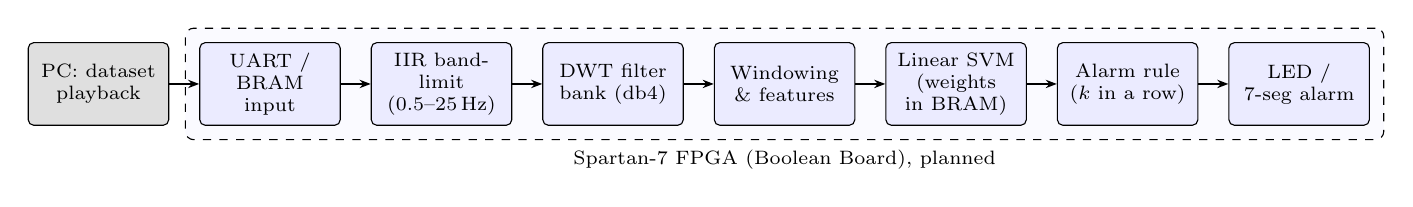
\begin{tikzpicture}[
  font=\scriptsize,
  blk/.style={draw, rounded corners=2pt, minimum height=1.05cm,
              text width=1.55cm, align=center, fill=blue!8},
  pcblk/.style={blk, fill=gray!25},
  arr/.style={-{Stealth[length=4pt]}, thick},
  node distance=0.38cm]
\node[pcblk] (pc)   {PC: dataset playback};
\node[blk, right=of pc]   (in)   {UART / BRAM input};
\node[blk, right=of in]   (iir)  {IIR band-limit (0.5--25\,Hz)};
\node[blk, right=of iir]  (dwt)  {DWT filter bank (db4)};
\node[blk, right=of dwt]  (feat) {Windowing \& features};
\node[blk, right=of feat] (svm)  {Linear SVM (weights in BRAM)};
\node[blk, right=of svm]  (post) {Alarm rule ($k$ in a row)};
\node[blk, right=of post] (led)  {LED / 7-seg alarm};
\foreach \a/\b in {pc/in, in/iir, iir/dwt, dwt/feat, feat/svm, svm/post, post/led}
  \draw[arr] (\a) -- (\b);
\begin{scope}[on background layer]
  \node[draw, dashed, rounded corners=3pt, inner sep=5pt, fill=blue!2,
        fit=(in)(iir)(dwt)(feat)(svm)(post)(led),
        label={[font=\scriptsize]below:Spartan-7 FPGA (Boolean Board), planned}] {};
\end{scope}
\end{tikzpicture}
\caption{Conceptual, proposed architecture. The shaded block runs on the
host PC; light-blue blocks are planned FPGA modules. No part of this
pipeline has been implemented at the time of writing.}
\label{fig:arch}
\end{figure*}

\begin{table*}[t]
\centering
\caption{Design decisions. The working baseline is the configuration the
software study starts from and ablates against; it is not a final
choice. Alternatives to be compared include 1--4\,s windows, 3--4 DWT
levels, a lifting-form DWT, per-patient channel selection, parallel
per-channel datapaths, log-energy features, and a small MLP if a linear
boundary proves inadequate.}
\label{tab:decisions}
\small
\begin{tabularx}{\textwidth}{@{}p{3.2cm}X@{}}
\toprule
Decision & Working baseline \\
\midrule
Channels & Common bipolar subset present in all recordings used (fixed after montage inspection; at most 23) \\
Window / hop & 2\,s window as in \cite{shoeb2010icml}; 1\,s hop \\
Band-limit & 0.5--25\,Hz as in \cite{shoeb2010icml}, IIR biquad cascade applied continuously \\
DWT & db4, 5 levels, direct-form filter pair \\
Features & Sub-band energy and line-length (Eqs.~\ref{eq:energy}, \ref{eq:ll}); variance or log-energy only if the baseline shows a benefit \\
Classifier & Linear SVM; weights fixed offline, stored in BRAM; class-weighted training \\
Numeric format & Fixed-point; word length $B$ swept and checked bit-exactly against the Python model \\
Channel processing & One time-multiplexed engine shared across channels, per-channel state in BRAM \\
Post-processing & Alarm after $k$ consecutive positive windows; initial $k=3$, tuned on validation data \\
Input interface & PC to FPGA over UART at 230\,400 baud \\
Evaluation & Patient-specific, leave-one-record-out. Subjects: the first three cases
in numeric order with at least 3 annotated seizures and a 23-channel
bipolar montage common to all their files (checked in the per-case
summary files). Only one of chb01/chb21 (same subject) is eligible. \\
\bottomrule
\end{tabularx}
\end{table*}

\paragraph{Input path.} The real EEG front-end is not part of the initial
scope: scalp EEG is microvolt-level and noisy, and acquiring it
introduces a very different risk profile from playback. An offline EEG
dataset will instead be streamed to the FPGA to emulate a real-time
input. Streaming 23 channels of 16-bit data at 256\,Hz requires
$23\times2\times256=11{,}776$\,bytes/s, which with 8N1 framing (10 bits
per byte) is 117,760\,baud and exceeds the standard 115,200\,baud rate.
The UART will therefore be configured at 230,400\,baud, which we will
confirm against the board's USB-to-UART bridge specification
\cite{realdigital2024boolean}, or fewer channels will be used. Selected
seizure and non-seizure segments will be pre-converted offline into a
hardware-friendly fixed-point format and stored either via streaming
playback or in on-chip block RAM; a faster-than-real-time playback mode
will be used for testing.

\paragraph{Processing chain.} The continuous pipeline is an IIR biquad
band-pass, a 5-level db4 DWT, then windowing and feature accumulation,
followed by the linear SVM and temporal post-processing. Filtering and
the DWT run continuously, sample by sample, as pipelines; windowing is
applied only when accumulating features, so filter state is not
restarted per window and there are no window-edge transients. The
alarm delay is approximately $T + d_{\mathrm{DWT}} + (k-1)h$ for window
length $T$, hop $h$, and a causal DWT delay $d_{\mathrm{DWT}}\le
7(2^{J}-1)/f_s$ (about 0.85\,s for $J=5$ at 256\,Hz), which sets the
latency budget $\tau$ in Eq.~\eqref{eq:problem}.

\paragraph{Fixed-point arithmetic and quantization.} The translation
from software to hardware introduces quantization noise. Uniform
quantization with $B$ bits and step $\Delta$ adds noise power
$\Delta^{2}/12$, giving $\mathrm{SQNR}\approx6.02B+1.76$\,dB for a
full-scale sinusoid; EEG uses a smaller part of the range, so the
effective SQNR is lower. The worst-case $\ell_\infty$ gain of an FIR
stage is its $\ell_1$ norm. For the db4 analysis filters
$\|h\|_1=\|g\|_1\approx1.87<2$, so the level-$j$ output is bounded by
$1.87^{j}$ times the input peak and one guard bit per level suffices
within the DWT. This is a worst-case bound and covers the DWT only.
Over $N_b$ samples, the line-length accumulator needs
$B+1+\lceil\log_2 N_b\rceil$ bits and the energy accumulator
$2B+\lceil\log_2 N_b\rceil$ bits (Sec.~\ref{sec:features}); products are
truncated before accumulation to fit the $25\times18$ DSP48E1
multipliers. The IIR band-pass needs separate care: for a 0.5\,Hz corner
at 256\,Hz its poles lie close to the unit circle, so its gain and its
sensitivity to coefficient quantization will be measured and reported in
the word-length study. If this proves impractical, fallbacks are a
gentler high-pass corner or filtering after decimation. The word length
$B$ will be swept as an experimental variable and verified bit-exactly
against a fixed-point Python reference model.

\paragraph{Post-processing.} A single positive window can be caused by
a brief artefact or a benign burst that resembles seizure onset. Shoeb
and Guttag \cite{shoeb2010icml} note that a detector can be made to
declare a seizure only when suspect activity persists, at the cost of
added latency, and that requiring longer evidence lowers the
false-detection rate while increasing latency. We therefore propose an
alarm rule that asserts only after $k$ consecutive positive windows; the
value of $k$ is not finalized and will be chosen on validation data.

\paragraph{Planned demonstration.} The final demonstration is intended
to stream pre-selected EEG segments from a PC to the board, process them
sample by sample, classify in real time, and show a seizure/no-seizure
indication on LEDs or the seven-segment display. This is a
dataset-playback demonstration, not a medically validated clinical
device, and we make no claim that it can diagnose epilepsy or safely
monitor a patient.

%---------------------------------------------------------------------
\section{Next Steps}
\label{sec:next}

Table~\ref{tab:plan} lays out the staged plan. Nothing in it has been
completed; all measurements listed are future work.

\begin{table*}[t]
\centering
\caption{Staged plan. All items are future work.}
\label{tab:plan}
\small
\begin{tabularx}{\textwidth}{@{}p{3.2cm}X@{}}
\toprule
Stage & Planned work \\
\midrule
Dataset preparation & Download the selected subjects; inspect per-case summary files for montage differences; determine a usable channel set; parse EDF files; extract annotated seizure intervals; build labelled windows with a chosen length and overlap. \\
Software baseline & Implement the IIR band-pass / pre-filter and the db4 DWT in Python; compute candidate features; train a linear SVM offline with class weighting or balanced sampling; fix the evaluation protocol (Sec.~\ref{sec:protocol}); validate on selected subjects using sensitivity, false detections per hour, and latency. \\
Reference model & Build a floating-point reference; choose a fixed-point representation and word lengths; quantify numerical error against the reference; define the expected hardware outputs. \\
FPGA design & Implement, in turn, the IIR band-pass filter, DWT filter bank, feature extraction, linear SVM, and post-processing; integrate a streaming interface (UART and/or BRAM playback); decide between parallel and time-multiplexed channel processing. \\
Verification & Compare Verilog outputs with the Python model (targeting bit-exact agreement of the fixed-point model); measure latency and throughput; record resource use (LUTs, DSP blocks, BRAM) and clock frequency; test representative seizure and non-seizure segments. \\
Final demonstration & PC-to-FPGA dataset streaming; live classification; LED or seven-segment indication; a written comparison with the published works in Table~\ref{tab:lit}, with protocol differences stated. \\
\bottomrule
\end{tabularx}
\end{table*}

% \paragraph{Timeline and roles.} Targets follow the course deadlines;
% owners are to be agreed within the team.
% \begin{itemize}
%   \item By 25 Oct (mid-term): dataset inspection, Python reference
%     (IIR, db4 DWT, features), linear-SVM baseline, and one replicated
%     published result. [TODO: owners]
%   \item By 8 Nov: fixed-point model and word-length sweep; Verilog
%     datapath, SVM, and UART/BRAM playback. [TODO: owners]
%   \item By 13 Nov (final): verification, resource and latency report,
%     demonstration on the board, and final report and code. [TODO: owners]
% \end{itemize}

\paragraph{Risks.} The first risk is data handling: EDF parsing and
non-uniform montages take time, even though only the selected subjects
need to be downloaded (Sec.~\ref{sec:dataset}). The second is protocol
choice, since results are only meaningful relative to a stated
evaluation (Sec.~\ref{sec:protocol}). The third is hardware fit: the
resource budget of the target FPGA will bound the channel count and the
feature set. The fourth is the fixed-point behaviour of the low-corner
IIR filter (Sec.~\ref{sec:arch}).

%---------------------------------------------------------------------
\section*{AI Tool Usage}

% TODO: this statement must be true and specific. Edit it to match what
% you actually did, and be ready to explain every AI-assisted part in the
% viva.
Generative AI (Claude Sonnet 5.5) was used in two ways.
(1) During topic selection, to compare candidate projects (ECG signal
processing, edge detection, noise cancellation) and to estimate
hardware feasibility on the Boolean Board. (2) To generate the initial
\LaTeX{} structure and section outlines of this report. The authors are responsible for the technical
content and can explain and defend it, including
Eq.~\eqref{eq:macs}, the bit-growth argument and the UART-rate
calculation. Cited works were checked against the publications where
full text was available; for \cite{shen2022dwt,shanmugam2025ffnn,%
feng2018vlsi,alam2024qda,wen2022asic} only abstracts or partial text
were accessible, and the corresponding fields are marked ``Not
verified'' in Table~\ref{tab:lit}. 
% [CONFIRM THIS LIST MATCHES WHAT YOU
% ACTUALLY CHECKED.]

%---------------------------------------------------------------------
{\small
\bibliographystyle{ieeenat_fullname}
% references.bib = your uploaded bib file; extra_refs.bib = the new entries
\bibliography{references}
}

\end{document}